\documentclass[10pt]{IEEEtran}
\usepackage{latexsym}
\usepackage{algorithm}
\usepackage{algpseudocode}
\usepackage{natbib}
\usepackage{graphicx}
\usepackage{subfigure}
\title{Action Selection in ASAMI}
\author{Shun Zhang}
\date{}

\begin{document}
\maketitle

%\begin{abstract}
%\end{abstract}

\section{Analysis of ASAMI}

The action model and sensor model of a robot can be learned
simultaneously without external feedback \cite{CSJ06}.  In the ASAMI
algorithm, actions are selected randomly in the training. However,
this can be biased according to the current belief.  In this sense,
the agent should be able to determine which action would lead to the
most uncertain results and thus need more samples.  The agent doesn't
know the correctness of the models. It only knows the consistency of
them. For example, states with larger difference in action model and
sensor model ($|W_a - W_s|$) should be considered as inconsistent.
Unobserved state, action pairs can be also assumed as inconsistent.

The first author of \cite{CSJ06}, Dan Stronger, commented that ``one
possible reason the $W_a$ is wrong after a certain action is that the
action is just very noisy \ldots This is a good reason to gather more
data for that action \ldots  But another possible reason  an action
could be causing problems is because the action model function being
fit, with the degrees of freedom that it has, just fits to a function
that's not especially accurate for that action''. This would be a
problem in degree selection in the polynomial regression, which is
discussed in \cite{IJAIT08-stronger}. In this report, I'll give our
action model proper degrees of freedom. So, if the action model is
inconsistent, the reason should be that either there are too few data
gathered to make consistency happen, or the data gathered are too
noisy.

\hfill

The action selection is even necessary in some environment. The
experiments in \cite{CSJ06} assume that \textit{we} know the effect
the actions -- for example, some actions would make it go forward, and
others make it go backward -- while the robot does not. So to explore
the environment, we make the robot walk forward and walk backward
alternatively to explore the state space. However, these the actions
may be totally unknown.  If the agent still chooses actions uniformly
random, then exploration would be low effecient.

For example we consider 1-dimensional walk. Let the world be in the
range of $[0,n]$. The agent starts at 0, and wants to reach $n$. Let
the range of velocity be $[-2a, 2a]$ (positive velocities mean going
forward, and negative ones mean going backward), and in every step the
agent chooses an action uniformly random.  Then, the expected absolute
velocity is $a$. Assume the agent would ``bump into'' the boundary of
$0$ and stays there if it tries to go backward from position $0$. The
expected \textit{moving forward} steps needed to take to reach
distance $n$ is $\frac{n}{a}$. This forms a \textit{random walk}
\cite{motwani1995randomized} problem. The expected steps needed to
take to reach distance $n$ is $O(n^2)$. This concludes that, if an
agent takes random actions in an unkown domain, it's likely that the
agent would confine itself in a small domain.

\section{Literature Review}

In the perspective of model-adaptive agents \cite{maes1993modeling},
This solves the problem of \textit{action selection}, as it
accelerates the progress towards its goal - consistency between action
model and transition model. This also solves the problem of
\textit{learning from experience}, as the inconsistency is an
essential information that can be used for further decision-making.

There is a two-dimensional version of ASAMI discussed in
\cite{ICRA08-stronger}.  As the action space is larger in higher
dimension, biasing on actions instead of random selection on actions
becomes more essential. The proposed approach can be proceeded if the
proposed modification works in one-dimensional environment.

Compared with this proposed method, some similar ideas are discussed
in the developmental robotics literature. They call the inconsistency
described above as \textit{error} \cite{oudeyer2006discovering},
\textit{surprise} \cite{ranasinghe2008surprise} or \textit{curiosity}
\cite{schmidhuber2006developmental}. This serves as a motivation to
change the model. A metric can be used to describe the global
inconsistency \cite{oudeyer2006discovering}. Then, a reinforcement
learning framework can be used to plan to get to the states with the
least global inconsistency. The authors in
\cite{ranasinghe2008surprise} used logic rules as the model, and let
the robot figure out why there could be a surprise. In this report, I
assume that the surprise is caused by insufficient or noisy data. So
the surprise, or inconsistency, of an action, is simply caused by the
data gathered at that action.

Additionally, there is an assumption in \cite{CSJ06} that there is a
mapping from action to the difference of state, i.e., $A \rightarrow
\Delta S$.  This is true in robot motion. So it's possible to learn
the difference in the observation, when the action is given. This is
exactly how the task is designed in \cite{ICDL10-hester}. If this is
not true, so that $S \times A \rightarrow S$ is the best we can
estimate, this would become more challenging but still possibly to be
dealt with. We might know that a certain $(s, a)$ is inconsistent and
we want to gather more data on it. But our action model might not be
well-learned. So the reward should be a compromise between the
inconsistency of that $(s, a)$ and the cost to reach it.

There are also other related works on learning the action model. But
they're using very different approach. They assume that one model,
usually the sensor model, is well calibrated. The data are represented
as either statistics \cite{And_learningand} or instances
\cite{LNAI2007-ahmadi}. These would be further analyzed and compared
with our approach in section \ref{sec:dis}.

\section{Proposed Algorithm}

In this section, I propose an algorithm, called Strong ASAMI, that
makes the agent choose action in a computationally cheap way. This can
be applied when there is no prior domain knowledge about them. The
idea is that we devide the learning into two phases. The agent leanrs
actions first and learns the state space later. In the frist
phase, it chooses the action with least confidence to learn. In the
second phase, it uses the actions it learned to explore the
environment.

Two essential functions are presented in Algorithm~\ref{alg:asami}. In
each iteration (frame for Nao), \textsc{update} is called to update
the knowledge on action effects. When the robot needs to decide which
is the next action to take, \textsc{getAction} is called.

The action selection strategy in phase 2 is quite vague. However, this
is up to the agent how to plan to traverse the state space. For
example, it might want to keep trying actions with positive $\Delta
Observation$ so that before reaching a boundary, and then go the
reverse way.

\begin{algorithm*}[t]
\caption{Strong ASAMI}\label{alg:asami}
\begin{algorithmic}
\Function{initialize}{$rangeOfActions$}
    \State $actions \gets$ discretified $rangeOfActions$
    \For{$action$ in $actions$}
        $samples[action] \gets \{\}$ \Comment{This will contain
	observations when $action$ is done}
    \EndFor
\EndFunction
\\
\Function{getAction}{} \Comment{This is called when the robot needs to
decide an action}
\State $trials\gets 0$
    \While {True}
        \If {$trials\leq$ ACTION\_LEARNING\_TRIALS}
            \State $action \gets$ the action such that $samples[action]$ has the largest variance
        \Else
            \State $action \gets$ appropriate action for state exploration
        \EndIf
        \State increase $trials$
    \EndWhile
\EndFunction
\\
\Function{update}{$action, \Delta observation$} \Comment{This is called when
each observation is retrieved.}
    \State add $\Delta bservation$ to $samples[action]$ \Comment{It's
    assumed that the change of observation is correlated to the
    action, not the absolute observation.}
\EndFunction
\end{algorithmic}
\end{algorithm*}

\section{Experiments}

\subsection{Test in Simulator}

\begin{figure}[h]
\centering
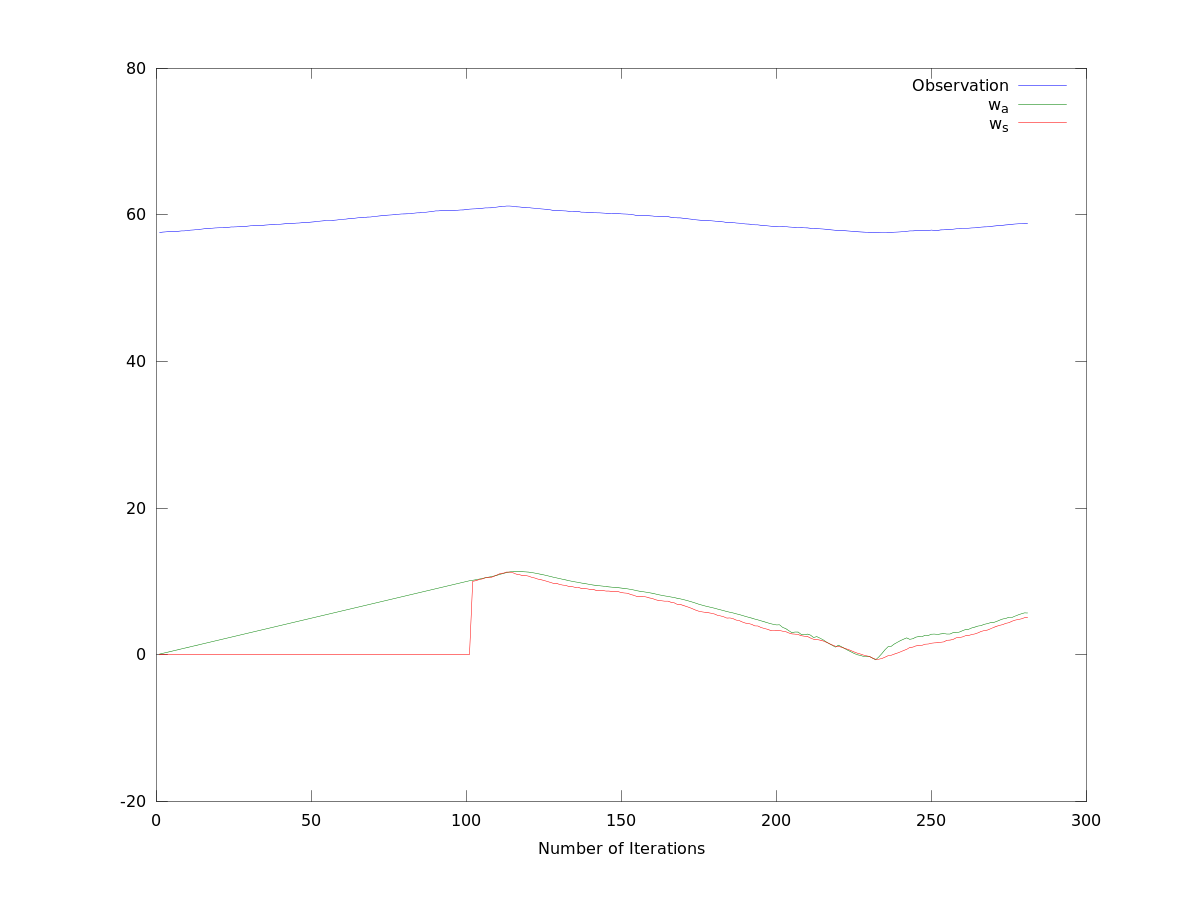
\includegraphics[width=\columnwidth]{simResult.png}
\caption{The Simulator.}
\label{fig:fuelworld}
\end{figure}


$T\_START$ = 10. $\lambda$ = 0.2. 

Action model and sensor model are both assumed to be cubic functions.
We have four parameters to estimate for each model.

\subsection{Test on Nao}

The challenges are that beacon height is too noisy.

\begin{figure}[h]
\centering
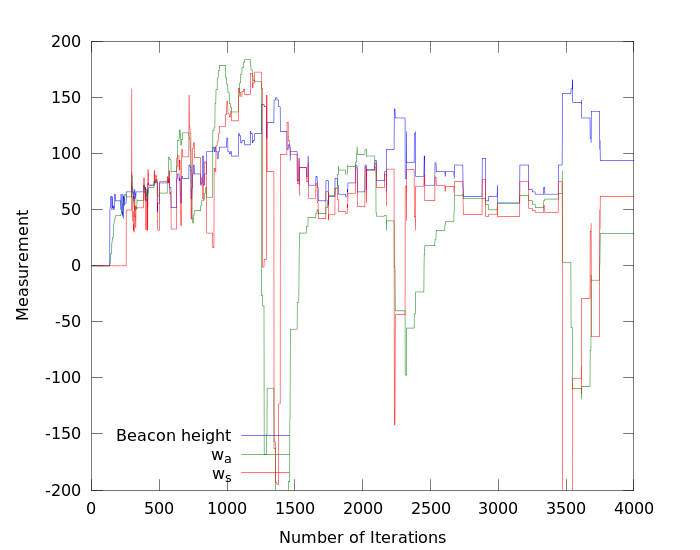
\includegraphics[width=\columnwidth]{demoResult.png}
\caption{Testing of ASAMI on Nao during the class demo. The
observation comes continuously (30 frames per second). Everytime the
robot changes from walking forward to warking backward (when the
height the beacon turns to decreasing). It's kidnapped at around 3,500
step.  (The colors are different from those in real-time plotting in
class)}

\label{fig:fuelworld}
\end{figure}


\section{Discussion and Conclusion}
\label{sec:dis}

It's possible that learning each discrete action independently would
have a better performance. Though it is interesting to estimate what
the most likely continuous model, expressed by polynomial function, by
the samples. It has several constraints. First, degree selection
should be determined, possibly using methods in
\cite{IJAIT08-stronger}. But the model many not be a small-dimensional
polynomial, so there might be too many parameters to estimate. Second,
the inherent drawback of function approximation method is that local
updates could have global effects. This is especially harmful in a
noisy environment.

%=====================================================================
\bibliographystyle{plain}

\bibliography{report}

\end{document}
